\documentclass{bioinfo2}

\copyrightyear{2015}
\pubyear{2015}

\usepackage{amsmath}
\usepackage{natbib}

\newcommand{\specialcell}[2][c]{%
  \begin{tabular}[#1]{@{}l@{}}#2\end{tabular}}

\usepackage{caption}
\renewcommand{\thetable}{S\arabic{table}}

\bibliographystyle{apalike}

\begin{document}
\firstpage{1}
\renewcommand{\thepage}{S\arabic{page}}

\title[Metagenome-enabled error correction]{corsage: Metagenome-enabled error correction of single cell sequencing reads}

\author[Bremges \textit{et~al.}]{Andreas Bremges\,$^{1}$\footnote{to whom correspondence should be addressed}, Esther Singer\,$^{2}$, Tanja Woyke\,$^{2}$ and Alexander Sczyrba\,$^{1}$}

\address{$^{1}$Center for Biotechnology \& Faculty of Technology, Bielefeld University, 33615 Bielefeld, Germany\\
$^{2}$U.S. Department of Energy Joint Genome Institute, Walnut Creek, CA 94598, USA}

\maketitle

\section{Single amplified genomes}

\textit{Descibe why and how the SAGs were generated. Cite \citep{scott2}. State average sequencing depth (constant), but different MDA quality levels. Highlight two exceptionally well amplified SAGs (6 \& 7), that are closer to isolate-grade genomes. Also highlight the problematic ones mentioned in main text, where the hybrid error correction clearly outperforms SAG-only correction. Table \textbf{S1}.}

\begin{table}[h]
\processtable{Per-base coverage for the eight \textit{E. coli} SAGs.}
{\footnotesize
%\begin{tabular}{p{1.1cm}p{1.5cm}p{1.4cm}p{1.5cm}p{1.4cm}} %.0
\begin{tabular}{lrrrrrrr}
\toprule
SAG  & mean & std.dev & min & max & Q1 & Q2 & Q3 \\
\midrule
0 & 289.749 & 486.983 & 0 & 6560 & 36 & 112 & 331 \\
1 & 297.379 & 386.285 & 0 & 4774 & 70 & 169 & 355 \\
2 & 272.085 & 708.577 & 0 & 12254 & 18 & 57 & 188 \\
3 & 260.303 & 762.898 & 0 & 16120 & 11 & 49 & 198 \\
4 & 284.087 & 783.65 & 0 & 13996 & 7 & 43 & 174 \\
6 & 266.821 & 275.48 & 3 & 3861 & 105 & 179 & 321 \\
7 & 278.141 & 241.48 & 4 & 2124 & 124 & 195 & 334 \\
8 & 299.661 & 399.265 & 0 & 4816 & 58 & 168 & 384 \\
\botrule
\end{tabular}}{Describe methods: mapping of raw reads with bwa mem~\citep{bwamem} then samtools to view, sort and depth~\citep{samtools} options of depth: -q0 -Q0 (with source code modified to remove the hardcoded coverage max).
bla bla}
\end{table}

\begin{figure}[t]
\centering
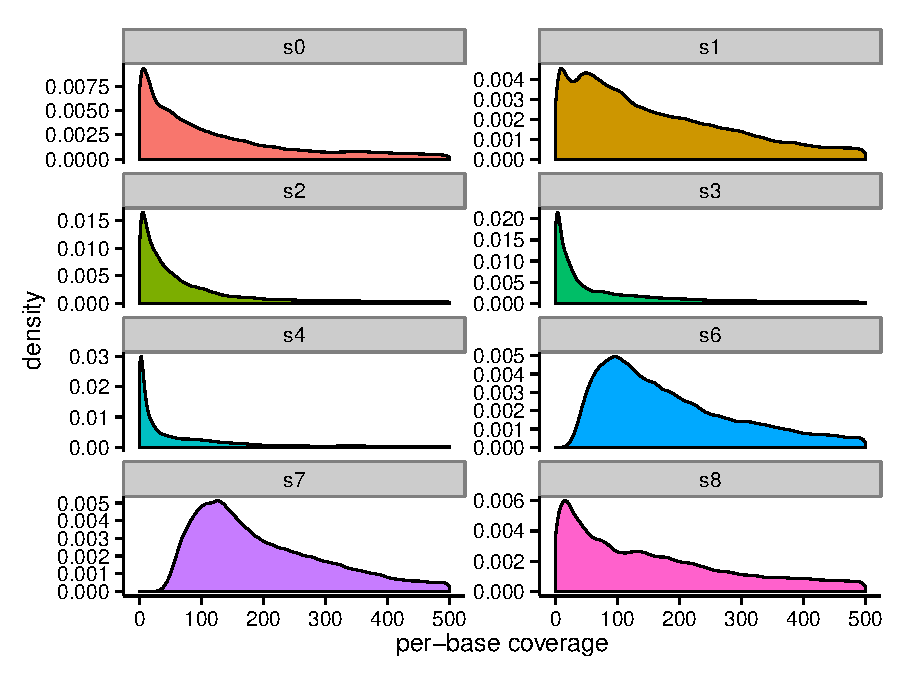
\includegraphics[width=.5\textwidth]{sag_depth}
\caption{Per-base coverage for the eight \textit{E. coli} SAGs.}
\end{figure}

\section{Mock metagenome}

\textit{Generated at the JGI, initially for internal benchmarking. NCBI accession number or some way to get it via IMG or GOLD (alternatively, might be okay to provide upon request, contact Tanja?). Describe what's in there. Refer to table with molecular weights and mapping statistics (genome coverage), Table \textbf{S2}.}

\textit{Probably also include a tree containing all 26 genomes, based on their 16S (or -- simpler -- extracted from iTOL, as all are known!). This might be of interest to see how closely related the stuff in there is. Discuss with others!}

\begin{figure*}[t]
\centering
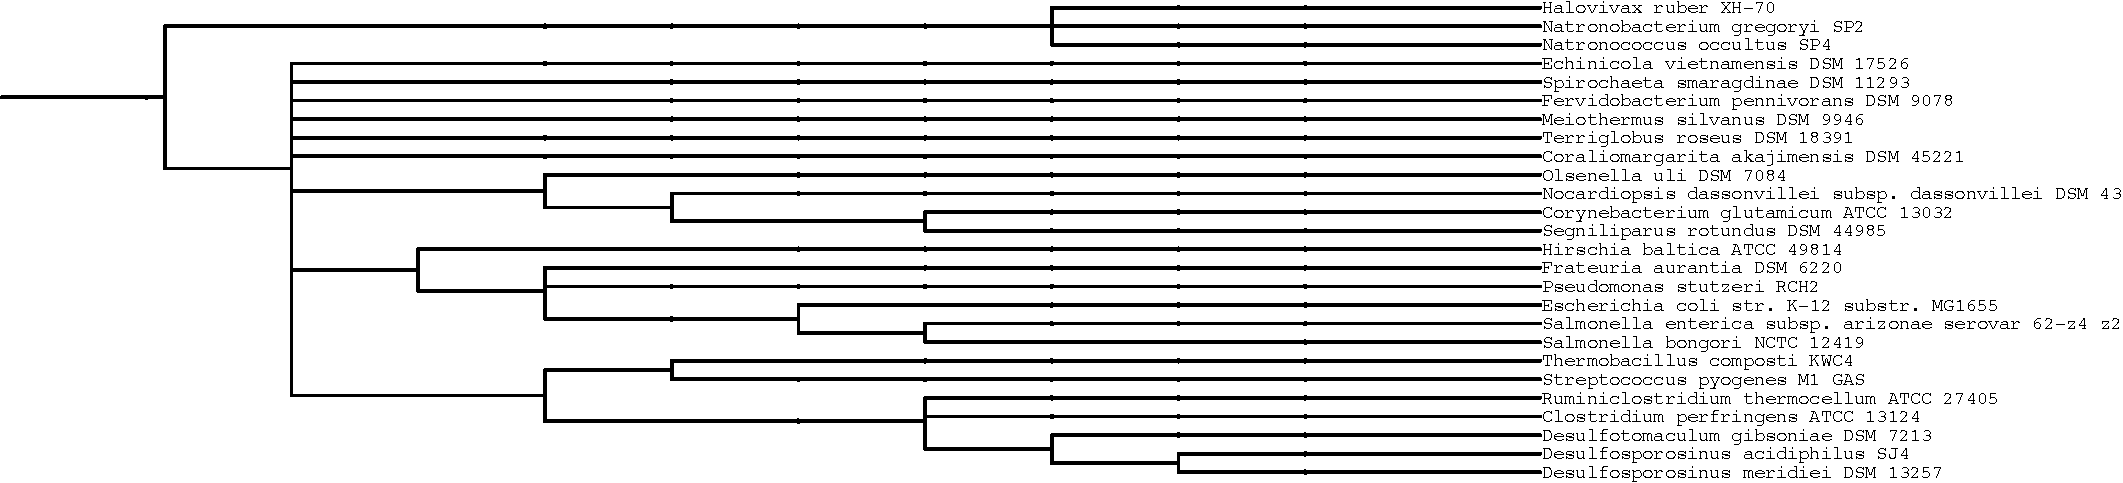
\includegraphics[width=\textwidth]{tree_normal}
\caption{phyloT/iTOL \citep{itol,itol2} phylogenetic tree of the 26 members of the mock metagenome.}
\end{figure*}

\section{Metrics per SAG}

\textit{Read-based in Table \textbf{S3}, assembly-based in Tables \textbf{S4} and \textbf{S5}.}

\textit{Explain the parameter sweep for -c, the metagenomic coverage threshold. Setting this to 2 already produces much better results, with a higher threshold yielding slightly better results, but more sample-specific. Setting it to 2 should work in all cases, and thus is the default setting. You might get better results if you play around with it, depends on target coverage in the metagenome.}

\textit{Assembly parameters (k) were tuned to maximize the NG50 value of the BayesHammer + SPAdes assembly. Changing from the default -k 21,33,55 to -k 21,33,55,77 produced better assemblies, thus we picked this combination. -{}-careful reduces the number of misassemblies by (1) less aggressive assemby and (2) polishing of the contigs in a postprocessing step involving read mapping.}

\bibliography{corsage_refs}

\begin{table*}[p]
\processtable{Profile of the mock metagenome.}
{\footnotesize
%\begin{tabular}{p{1.1cm}p{1.5cm}p{1.4cm}p{1.5cm}p{1.4cm}} %.0
\begin{tabular}{lrrrr}
\toprule
NCBI Taxonomy ID & Scientific name & ContigLength & MappedReads & AvgCoverage \\ %TODO Molarity
\midrule
646529 & Desulfosporosinus acidophilus SJ4 : Contig240.3 & 3897 & 367804 & 13410.8450089813 \\
&Desulfosporosinus acidophilus SJ4 : Contig241.2 & 60447 & 2309615 & 5644.16513640048 \\
&Desulfosporosinus acidophilus SJ4 : Contig243.1 & 4926837 & 50525496 & 1520.41947886646 \\
\hline
767817 & Desulfotomaculum gibsoniae DSM 7213 & 4855529 & 24329020 & 741.835021889479 \\
\hline
768704 & Desulfosporosinus meridiei DSM 13257 & 4873567 & 16066750 & 487.573607585573 \\
\hline
926556 & Echinicola vietnamensis DSM 17526 & 5608040 & 2160987 & 57.2232760465332 \\
\hline
771875 & Fervidobacterium pennivorans DSM 9078 & 2166381 & 39566833 & 2708.24050709455 \\
\hline
767434 & Frateuria aurantia DSM 6220 & 3603458 & 13922996 & 568.15908080516 \\
\hline
797302 & Halovivax ruber XH-70 & 3223876 & 6060380 & 274.952728640928 \\
\hline
511145 & Escherichia coli str. K-12 substr. MG1655 & 4639675 & 647555 & 20.6521661538793 \\
\hline
195103 & Clostridium perfringens ATCC 13124 & 3256683 & 1461840 & 66.5510195496461 \\
\hline
203119 & Clostridium thermocellum ATCC 27405 & 3843301 & 1542460 & 59.6166532363715 \\
\hline
582402 & Hirschia baltica ATCC 49814 & 3455622 & 27502745 & 1182.5057080896 \\
&Hirschia baltica ATCC 49814 plasmid pHbal01 & 84492 & 641481 & 1126.13552762392 \\
\hline
583355 & Coraliomargarita akajimensis DSM 45221 & 3750771 & 11810956 & 467.028614916773 \\
\hline
640132 & Segniliparus rotundus DSM 44985 & 3157527 & 4886507 & 225.630138079579 \\
\hline
446468 & Nocardiopsis dassonvillei subsp. dassonvillei DSM 43111 & 5767958 & 5761 & 0.0573058957780206 \\
&Nocardiopsis dassonvillei subsp. dassonvillei DSM 43111 plasmid pNDAS01 & 775354 & 879 & 0.0682900971685192 \\
\hline
526227 & Meiothermus silvanus DSM 9946 & 3249394 & 27813938 & 1261.46624232088 \\
&Meiothermus silvanus DSM 9946 plasmid pMESIL01 & 347854 & 3461768 & 1466.53106188228 \\
&Meiothermus silvanus DSM 9946 plasmid pMESIL02 & 124421 & 955914 & 1123.36214947637 \\
\hline
633147 & Olsenella uli DSM 7084 & 2051896 & 7839526 & 552.985752201866 \\
\hline
573413 & Spirochaeta smaragdinae DSM 11293 & 4653970 & 39431130 & 1255.9706035922 \\
\hline
797304 & Natronobacterium gregoryi SP2 & 3788356 & 8676937 & 335.230170554193 \\
\hline
694430 & Natronococcus occultus SP4 : Contig265 & 12939 & 243363 & 2564.16840559549 \\
&Natronococcus occultus SP4 : Contig266 & 287963 & 819298 & 396.405625028215 \\
&Natronococcus occultus SP4 : Contig267 & 4013216 & 11443075 & 397.25378947956 \\
\hline
644801 & Pseudomonas stutzeri RCH2 : Contig40.4 & 2804 & 62801 & 3135.38908701855 \\
&Pseudomonas stutzeri RCH2 : Contig44.3 & 9865 & 4321 & 64.2942726811961 \\
&Pseudomonas stutzeri RCH2 : Contig45.2 & 12763 & 54681 & 630.421844393951 \\
&Pseudomonas stutzeri RCH2 : Contig47.1 & 4575057 & 5326365 & 171.651879965649 \\
\hline
926566 & Terriglobus roseus DSM 18391 & 5227858 & 8464573 & 239.329327805002 \\
\hline
717605 & Thermobacillus composti KWC4 : Contig54.2 & 149182 & 1912248 & 1900.01226689547 \\
&Thermobacillus composti KWC4 : Contig56.1 & 4206343 & 29042078 & 1016.11924491179 \\
\hline
160490 & Streptococcus pyogenes M1 GAS & 1852441 & 1502208 & 120.443499145182 \\
\hline
882884 & Salmonella enterica subsp. arizonae serovar 62:z4,z23:- str. RSK2980 & 4600800 & 1831145 & 58.7192305685968 \\
\hline
218493 & Salmonella bongori NCTC 12419 & 4460105 & 501312 & 16.60908140055 \\
\hline
196627 & Corynebacterium glutamicum ATCC 13032 & 3309401 & 1063668 & 47.6651768703762 \\
\botrule
\end{tabular}}{Describe methods: mapping of raw reads with bwa mem \citep{bwamem} then samtools \citep{samtools},
input from Esther is needed. 
Total of 355875608 reads (53381341200bp) sequenced.
}
\end{table*}

\begin{table*}[p]
\processtable{Performance of error correction}
{\footnotesize
\begin{tabular}{llrrrrrrrr}
\toprule
Metric   & Program     & 0       & 1       & 2       & 3       & 4       & 6       & 7       & 8 \\
\midrule
Reads    & --          & 9365134 & 9604918 & 8811278 & 8396488 & 9257066 & 8609900 & 8990744 & 9682468 \\
\midrule
Perfect  & raw         & 2120932 & 2179609 & 1937541 & 1954244 & 1872800 & 2049675 & 2063874 & 2183454 \\
         & hammer      & 7656274 & 8260510 & 6302861 & 5970186 & 6297298 & 7639715 & 8068555 & 8317006 \\
         & corsage -c1 & 8276184 & 8578469 & 7861670 & 7433499 & 8192894 & 7736330 & 8046250 & 8656282 \\
         & corsage -c2 & 8886436 & 9188854 & 8440502 & 7965810 & 8829995 & 8264229 & 8611867 & 9272559 \\
         & corsage -c3 & 8965114 & 9270617 & 8511335 & \textbf{8024365} & 8904161 & 8330927 & 8683349 & 9347321 \\
         & corsage -c4 & \textbf{8974388} & \textbf{9278745} & \textbf{8511843} & 8023150 & \textbf{8910290} & \textbf{8338543} & \textbf{8689922} & \textbf{9354172} \\
         & corsage -c5 & 8943102 & 9243789 & 8471748 & 7993790 & 8875735 & 8310857 & 8654540 & 9312765 \\
\midrule
Chimeric & raw         &   69568 &   67625 &   81938 &   75509 &   79443 &   52246 &   44983 &   59265 \\
         & hammer      &   72820 &   70590 &   87564 &   80336 &   84813 &   53875 &   46387 &   61948 \\
         & corsage -c1 &   15129 &   13376 &   18281 &   12859 &   13501 &   10913 &    9954 &   12303 \\
         & corsage -c2 &    5502 &    4593 &   10397 &    4648 &    5257 &    3941 &    3824 &    4889 \\
         & corsage -c3 &    \textbf{5224} &    \textbf{4245} &   \textbf{10181} &    \textbf{4349} &    4802 &    \textbf{3642} &    \textbf{3555} &    \textbf{4614} \\
         & corsage -c4 &    5239 &    4247 &   10230 &    4881 &    \textbf{4777} &    3656 &    3558 &    4646 \\
         & corsage -c5 &    5318 &    4350 &   10321 &    4703 &    4896 &    3698 &    3611 &    4731 \\
\midrule
Better   & raw         & -- & -- & -- & -- & -- & -- & -- & -- \\
         & hammer      & 6743983 & 7026478 & 6156387 & 5669978 & 6574627 & 6244274 & 6645542 & 7095951 \\
         & corsage -c1 & 6899557 & 7131162 & 6610328 & 6169861 & 7102763 & 6311717 & 6653538 & 7200704 \\
         & corsage -c2 & 7008163 & 7236195 & 6707136 & \textbf{6260408} & 7206731 & 6403639 & 6749255 & 7306961 \\
         & corsage -c3 & \textbf{7017190} & \textbf{7247251} & \textbf{6715402} & 6258028 & \textbf{7215037} & \textbf{6412774} & \textbf{6759006} & \textbf{7315526} \\
         & corsage -c4 & 7011329 & 7242576 & 6709552 & 6238573 & 7211254 & 6408499 & 6753669 & 7310524 \\
         & corsage -c5 & 6987270 & 7218080 & 6681337 & 6211648 & 7184655 & 6388594 & 6729406 & 7280437 \\
\midrule
Worse    & raw         & -- & -- & -- & -- & -- & -- & -- & -- \\
         & hammer      &   31644 &   26951 &   32315 &   29096 &   41584 &   25270 &   26959 &   28960 \\
         & corsage -c1 &   76694 &   76914 &   65596 &   75134 &   75213 &   62950 &   65427 &   73162 \\
         & corsage -c2 &   25990 &   25304 &   20560 &   27335 &   27390 &   20791 &   21074 &   24001 \\
         & corsage -c3 &   21353 &   20867 &   17696 &   \textbf{23556} &   23768 &   17299 &   17238 &   20241 \\
         & corsage -c4 &   \textbf{20967} &   \textbf{20559} &   17040 &   24583 &   \textbf{23721} &   \textbf{17037} &   \textbf{16932} &   \textbf{20007} \\
         & corsage -c5 &   21386 &   21512 &   \textbf{16922} &   25583 &   24349 &   17529 &   17774 &   20919 \\
\midrule
Time    & hammer      &  \\
        & corsage     &  \\
\midrule
RAM    & hammer      &  \\
       & corsage     &  \\
\botrule
\end{tabular}}
{A read is said to become \emph{better} (or \emph{worse}) if the best alignment of the corrected sequence has more (or fewer) identical bases to the reference genome than the best alignment of the original sequence.
The table gives the number of reads mapped \emph{perfectly}, number of \emph{chimeric} reads (i.e. reads with parts mapped to different places), number of corrected reads becoming \emph{better} and the number of corrected reads becoming \emph{worse} than the original reads.
Mapping of raw and corrected reads to reference with BWA-MEM-0.7.12~\citep{bwamem}, postprocessing with samtools-1.2~\citep{samtools} and some custom scripts, all available on GitHub eventually.} %TODO Insert GitHub URL
\end{table*}

\begin{table*}[p]
\processtable{IDBA-UD assemby statistics}
{\footnotesize
\begin{tabular}{llrrrrrrrr}
\toprule
Metric & Program & 0 & 1 & 2 & 3 & 4 & 6 & 7 & 8 \\
\midrule
NG50 & raw     & 45284 & 53863 & 31250 & 24834 & 17196 & 87102 & 80574 & 59754 \\
     & hammer  & 40924 & 51004 & 29256 & 24023 & 17246 & \textbf{95532} & \textbf{87102} & 44292 \\
     & corsage & \textbf{59081} & \textbf{73496} & \textbf{54946} & \textbf{41749} & \textbf{31569} & 90184 & 80997 & \textbf{80997} \\
\midrule
\# contigs & raw     & 330 & 342 & 514 & 607 & 654 & 201 & 200 & 303 \\
           & hammer  & 335 & 345 & 530 & 626 & 653 & \textbf{191} & \textbf{194} & 328 \\
           & corsage & \textbf{277} & \textbf{272} & \textbf{409} & \textbf{497} & \textbf{512} & 200 & 198 & \textbf{249} \\
\midrule
Largest contig &    raw  & 227106 & 203026 & \textbf{203098} & 141383 & 102074 & \textbf{221687} & \textbf{232585} & 162612 \\
               & hammer  & 203098 & 157125 & 197417 & 141494 & 107872 & \textbf{221687} & 178322 & 139398 \\
               & corsage & \textbf{236473} & \textbf{203098} & 144213 & \textbf{141579} & \textbf{124628} & 221683 & 221683 & \textbf{236473} \\
\midrule
Total length & raw     & 4400079 & 4587934 & 4400469 & 4139052 & 3940625 & 4640153 & \textbf{4639167} & 4533515 \\
             & hammer  & 4402128 & \textbf{4591089} & 4400334 & 4144742 & 3934141 & \textbf{4641409} & 4638005 & \textbf{4538546} \\
             & corsage & \textbf{4408926} & 4590112 & \textbf{4421966} & \textbf{4171137} & \textbf{3972787} & 4639453 & 4636457 & 4538141 \\
\midrule
\# misassemblies & raw     & 16 & 11 & 15 & 32 & 36 & \textbf{0} & \textbf{0} & 10 \\
                 & hammer  & 17 & 11 &  9 & 37 & 37 & \textbf{0} & \textbf{0} &  8 \\
                 & corsage &  \textbf{9} &  \textbf{4} &  \textbf{2} & \textbf{13} & \textbf{20} & \textbf{0} & \textbf{0} &  \textbf{7} \\
\midrule
\# mismatches per 100 kbp & raw     & \textbf{4.17} & \textbf{3.64} & 10.16 & 17.02 & 20.41 & 0.31 & 0.13 & 3.16 \\
                          & hammer  & 4.88 & 3.88 & 12.50 & 16.35 & 20.76 & \textbf{0.15} & \textbf{0.11} & \textbf{2.90} \\
                          & corsage & 4.38 & 3.80 &  \textbf{7.93} &  \textbf{8.86} & \textbf{12.82} & 2.30 & 2.39 & 3.27 \\
\midrule
\# indels per 100 kbp & raw     & 0.32 & \textbf{0.24} & 0.69 & 1.47 & 1.09 & 0.13 & \textbf{0.09} & 0.36 \\
                      & hammer  & 0.32 & 0.29 & 0.79 & 1.52 & 1.51 & 0.11 & \textbf{0.09} & 0.34 \\
                      & corsage & \textbf{0.25} & 0.31 & \textbf{0.53} & \textbf{0.90} & \textbf{0.85} & \textbf{0.09} & \textbf{0.09} & \textbf{0.18} \\
\midrule
Genome fraction (\%) & raw     & 93.656 & 97.182 & 93.344 & 87.892 & 83.101 & 98.266 & 98.245 & 96.104 \\
                     & hammer  & 93.631 & 97.165 & 93.304 & 87.924 & 82.958 & 98.211 & 98.175 & 96.028 \\
                     & corsage & \textbf{93.928} & \textbf{97.431} & \textbf{93.988} & \textbf{88.827} & \textbf{84.053} & \textbf{98.271} & \textbf{98.252} & \textbf{96.265} \\
\midrule
\# genes & raw     & 3873 & 4049 & 3741 & 3477 & 3220 & 4186 & 4191 & 4027 \\
         & hammer  & 3859 & 4052 & 3709 & 3469 & 3208 & 4194 & 4199 & 4005 \\
         & corsage & \textbf{3931} & \textbf{4126} & \textbf{3857} & \textbf{3593} & \textbf{3347} & \textbf{4204} & \textbf{4202} & \textbf{4088} \\
\midrule
NGA50 & raw     & 44890 & 53863 & 31250 & 24224 & 16220 & 87102 & 80574 & 59589 \\
      & hammer  & 40924 & 51004 & 29207 & 24023 & 17227 & \textbf{95444} & \textbf{87102} & 44292 \\
      & corsage & \textbf{59081} & \textbf{73496} & \textbf{54946} & \textbf{41749} & \textbf{31567} & 90184 & 80997 & \textbf{80574} \\
\midrule
Time    & raw         &  \\
        & hammer      &  \\
        & corsage     &  \\
\midrule
RAM    & raw         &  \\
       & hammer      &  \\
       & corsage     &  \\
\botrule
\end{tabular}}
{\textbf{IDBA-UD}. Explain metric definitions as outlined by QUAST. State, that everything was computed with QUAST~\citep{quast}, default settings, contigs greater than 500bp, bla bla. Availability in GitHub.} %TODO Insert GitHub URL
\end{table*}

\begin{table*}[p]
\processtable{SPAdes assemby statistics}
{\footnotesize
\begin{tabular}{llrrrrrrrr}
\toprule
Metric & Program & 0 & 1 & 2 & 3 & 4 & 6 & 7 & 8 \\
\midrule
NG50 & raw     & 65444 & 95218 & 66287 & 48903 & 26823 & 114661 & 117715 & 86966 \\
     & hammer  & \textbf{86625} & 95218 & 67436 & 52817 & 31448 & \textbf{120770} & \textbf{132608} & 105995 \\
     & corsage & \textbf{86625} & \textbf{95517} & \textbf{72055} & \textbf{53947} & \textbf{36236} & 112350 & \textbf{132608} & \textbf{112853} \\
\midrule
\# contigs & raw     & 447 & 400 & 606 & 718 & 813 & 245 & 233 & 324 \\
           & hammer  & 302 & \textbf{275} & 474 & 594 & 676 & \textbf{198} & \textbf{185} & \textbf{250} \\
           & corsage & \textbf{288} & 279 & \textbf{418} & \textbf{534} & \textbf{569} & 210 & 213 & 263 \\
\midrule
Largest contig &    raw  & 203603 & \textbf{224667} & \textbf{218793} & \textbf{178300} & 113773 & 269308 & 268816 & 223154 \\
               & hammer  & \textbf{204882} & 203257 & \textbf{218793} & 167410 & 135551 & \textbf{312119} & 269348 & \textbf{269318} \\
               & corsage & 203394 & 224320 & \textbf{218793} & 178231 & \textbf{155221} & 268535 & \textbf{312008} & 268327 \\
\midrule
Total length & raw     & \textbf{4522153} & \textbf{4703061} & \textbf{4533214} & \textbf{4290463} & \textbf{4138591} & \textbf{4713277} & \textbf{4718163} & \textbf{4633297} \\
             & hammer  & 4443696 & 4633876 & 4464269 & 4233011 & 4046113 & 4686582 & 4689565 & 4584513 \\
             & corsage & 4452849 & 4645907 & 4471868 & 4240428 & 4065827 & 4698390 & 4702810 & 4600454 \\
\midrule
\# misassemblies & raw     & 15 & 2 & 22 & 45 & 51 & \textbf{1} & 3 & 12 \\
                 & hammer  & 11 & 7 & 19 & 31 & 38 & \textbf{1} & 2 & 7 \\
                 & corsage & \textbf{6} & \textbf{3} & \textbf{10} & \textbf{23} & \textbf{22} & \textbf{1} & \textbf{0} & \textbf{6} \\
\midrule
\# mismatches per 100 kbp & raw     & 15.30 & 11.57 & 34.70 & 48.21 & 50.53 & 2.84 & \textbf{2.14} & 9.72 \\
                          & hammer  & 12.70 & 10.30 & 30.34 & 40.41 & 48.42 & \textbf{1.27} & 2.17 & \textbf{7.66} \\
                          & corsage & \textbf{10.41} &  \textbf{9.32} & \textbf{22.69} & \textbf{30.86} & \textbf{36.47} & 5.66 & 5.21 & 8.43 \\
\midrule
\# indels per 100 kbp & raw     & 0.89 & 1.17 & 2.26 & 4.48 & 4.24 & 0.31 & \textbf{0.22} & 1.00 \\
                      & hammer  & 1.17 & 1.19 & 3.16 & 3.48 & 4.58 & \textbf{0.24} & 0.35 & 0.94 \\
                      & corsage & \textbf{0.64} & \textbf{0.95} & \textbf{2.24} & \textbf{3.30} & \textbf{3.28} & 0.55 & 0.31 & \textbf{0.83} \\
\midrule
Genome fraction (\%) & raw     & \textbf{94.241} & \textbf{97.948} & \textbf{94.239} & 89.098 & 84.372 & \textbf{98.665} & \textbf{98.708} & \textbf{96.702} \\
                     & hammer  & 94.050 & 97.527 & 93.984 & 89.133 & 84.220 & 98.505 & 98.446 & 96.459 \\
                     & corsage & 94.223 & 97.629 & 94.223 & \textbf{89.543} & \textbf{84.798} & 98.580 & 98.541 & 96.603 \\
\midrule
\# genes & raw     & 3876 & 4117 & 3782 & 3532 & 3281 & 4217 & \textbf{4224} & 4081 \\
         & hammer  & 3898 & 4124 & 3805 & 3562 & 3300 & 4211 & 4219 & 4093 \\
         & corsage & \textbf{3937} & \textbf{4133} & \textbf{3866} & \textbf{3608} & \textbf{3390} & \textbf{4218} & 4220 & \textbf{4097} \\
\midrule
NGA50 & raw     & 65444 & 95218 & 66287 & 41757 & 26823 & 114661 & 117715 & 86966 \\
      & hammer  & 82361 & 95218 & 67436 & 51035 & 31446 & \textbf{120770} & \textbf{132608} & 99558 \\
      & corsage & \textbf{86625} & \textbf{95435} & \textbf{71474} & \textbf{52883} & \textbf{36219} & 112350 & \textbf{132608} & \textbf{105926} \\
\midrule
Time    & raw         &  \\
        & hammer      &  \\
        & corsage     &  \\
\midrule
RAM    & raw         &  \\
       & hammer      &  \\
       & corsage     &  \\
\botrule
\end{tabular}}
{\textbf{SPAdes -{}-sc -{}-only-assembler -k 21,33,55,77 -{}-careful}. Explain metric definitions as outlined by QUAST. State, that everything was computed with QUAST, cite it, default settings, contigs greater than 500bp, bla bla. Availability in GitHub.} %TODO Insert GitHub URL
\end{table*}

\end{document}
